\PassOptionsToPackage{unicode=true}{hyperref} % options for packages loaded elsewhere
\PassOptionsToPackage{hyphens}{url}
%
\documentclass[
]{book}
\usepackage{lmodern}
\usepackage{amssymb,amsmath}
\usepackage{ifxetex,ifluatex}
\ifnum 0\ifxetex 1\fi\ifluatex 1\fi=0 % if pdftex
  \usepackage[T1]{fontenc}
  \usepackage[utf8]{inputenc}
  \usepackage{textcomp} % provides euro and other symbols
\else % if luatex or xelatex
  \usepackage{unicode-math}
  \defaultfontfeatures{Scale=MatchLowercase}
  \defaultfontfeatures[\rmfamily]{Ligatures=TeX,Scale=1}
\fi
% use upquote if available, for straight quotes in verbatim environments
\IfFileExists{upquote.sty}{\usepackage{upquote}}{}
\IfFileExists{microtype.sty}{% use microtype if available
  \usepackage[]{microtype}
  \UseMicrotypeSet[protrusion]{basicmath} % disable protrusion for tt fonts
}{}
\makeatletter
\@ifundefined{KOMAClassName}{% if non-KOMA class
  \IfFileExists{parskip.sty}{%
    \usepackage{parskip}
  }{% else
    \setlength{\parindent}{0pt}
    \setlength{\parskip}{6pt plus 2pt minus 1pt}}
}{% if KOMA class
  \KOMAoptions{parskip=half}}
\makeatother
\usepackage{xcolor}
\IfFileExists{xurl.sty}{\usepackage{xurl}}{} % add URL line breaks if available
\IfFileExists{bookmark.sty}{\usepackage{bookmark}}{\usepackage{hyperref}}
\hypersetup{
  pdftitle={A Person-Centered Framework},
  pdfauthor={Various authors},
  pdfborder={0 0 0},
  breaklinks=true}
\urlstyle{same}  % don't use monospace font for urls
\usepackage{longtable,booktabs}
% Allow footnotes in longtable head/foot
\IfFileExists{footnotehyper.sty}{\usepackage{footnotehyper}}{\usepackage{footnote}}
\makesavenoteenv{longtable}
\usepackage{graphicx,grffile}
\makeatletter
\def\maxwidth{\ifdim\Gin@nat@width>\linewidth\linewidth\else\Gin@nat@width\fi}
\def\maxheight{\ifdim\Gin@nat@height>\textheight\textheight\else\Gin@nat@height\fi}
\makeatother
% Scale images if necessary, so that they will not overflow the page
% margins by default, and it is still possible to overwrite the defaults
% using explicit options in \includegraphics[width, height, ...]{}
\setkeys{Gin}{width=\maxwidth,height=\maxheight,keepaspectratio}
\setlength{\emergencystretch}{3em}  % prevent overfull lines
\providecommand{\tightlist}{%
  \setlength{\itemsep}{0pt}\setlength{\parskip}{0pt}}
\setcounter{secnumdepth}{5}
% Redefines (sub)paragraphs to behave more like sections
\ifx\paragraph\undefined\else
  \let\oldparagraph\paragraph
  \renewcommand{\paragraph}[1]{\oldparagraph{#1}\mbox{}}
\fi
\ifx\subparagraph\undefined\else
  \let\oldsubparagraph\subparagraph
  \renewcommand{\subparagraph}[1]{\oldsubparagraph{#1}\mbox{}}
\fi

% set default figure placement to htbp
\makeatletter
\def\fps@figure{htbp}
\makeatother

\usepackage{booktabs}
\usepackage[]{natbib}
\bibliographystyle{apalike}

\title{A Person-Centered Framework}
\author{Various authors}
\date{2020-03-25}

\begin{document}
\maketitle

{
\setcounter{tocdepth}{1}
\tableofcontents
}
\hypertarget{reason}{%
\chapter{Reason}\label{reason}}

This framework comes from a simple starting point: the intent of supports and services is to help each person to flourish, to achieve a better life.

That belief is, thankfully, not a new one. It aligns with the MDHHS person-centered planning policy, which begins by stating that:\footnote{MDHHS BHDDA Person-Centered Planning Policy (June 5, 2017), p.~1}

\begin{quote}
\emph{The purpose of the community mental health system is to support adults and children\ldots{} to live successfully in their communities --- achieving community inclusion and participation, independence, and productivity {[}and to{]} to identify and achieve their personal goals.}
\end{quote}

The framework defined below is an attempt to apply these longstanding and fundamental values in a way that allows for consistent definitions, implementation, and evaluation.

\hypertarget{goal}{%
\section{Goal}\label{goal}}

Each person's ability to choose a better future and map their journey toward it: this is what person-centered planning enables. In order for services to effectively support a person in this process, they must be provided within the context of a person's goals. Orienting a broad and complex system to keep the person at the center requires a consistent, overarching framework. MDHHS BHDDA is working to support this person-centered orientation with the following strategy:

\textbf{Goal:} To develop \protect\hyperlink{bok}{a common body of knowledge} for person-centered planning,
mapped to \protect\hyperlink{policy}{relevant policies} and \protect\hyperlink{research}{research},
which will inform a \protect\hyperlink{curriculum}{shared curriculum}
and \protect\hyperlink{measure}{measurement framework}
to support \protect\hyperlink{pcpdca}{improved quality of life} for each person.

\hypertarget{pcpdca}{%
\chapter{Person-Centered Planning (Doing, Checking, Acting)}\label{pcpdca}}

The collective effect of our needs and environments has a profound impact on society, but the primary catalyst for transformation is at the level of the individual person. This is the profound insight of \emph{person-centered planning} (PCP), which has long been the cornerstone of Michigan policy related to behavioral health services and supports.\footnote{See the Michigan Mental Health Code, \href{http://legislature.mi.gov/doc.aspx?mcl-330-1712}{Act 258 of 1974, Section 330.1712}.}

Despite the central position of PCP to the Medicaid services system in Michigan, in practice it has often been relegated to the planning meeting itself and the preparation for that meeting: ensuring inclusion of family and friends, personal involvement, etc. While the act of developing a plan remains a cornerstone of the process, it is only the first step of what is needed to truly achieve one's goals.\footnote{Part of the focus on the meeting is due to the auditing focus on the plan document: an instance of \emph{what is measured, is addressed}.}

In this document and in the work under development with MDHHS-BHDDA, the phrase \emph{person-centered planning} is used broadly, to encompass not only the initial planning process but also its implementation, monitoring, and refinement. The need for this definition to extend beyond the PCP meetings and to direct all services and supports is already recognized within state policy, which indicates that:\footnote{MDHHS BHDDA Person-Centered Planning Policy (June 5, 2017), p.~1}

\begin{quote}
\emph{through PCP, a person is engaged in decision-making, problem solving, monitoring progress, and making needed adjustments to goals and supports and services provided in a timely manner.}
\end{quote}

Since the intent of supports and services is to improve personal quality of life, practitioners can view the PCP process as similar to the \emph{Plan-Do-Check-Act} (PDCA) cycle, which involves each element of the broad scope of PCP defined above. Versions of the PDCA cycle have already been successfully incorporated into the supports and treatment planning process for people with varying conditions and needs, from intellectual and developmental disabilities, to mental illness, to physical health concerns.

If we want to understand whether an individual person's plan is supporting their goals, it is necessary to have a strategy to measure improvement in the person's desired areas of focus. Such measurement-based approaches have been gaining traction in their use across populations.\footnote{\href{https://aaidd.org/docs/default-source/sis-docs/changes-in-the-field.pdf?sfvrsn=cd8b3021_0}{Shalock, et al.~(2018)} note ``an increased emphasis on\ldots{} conducting outcome evaluation\ldots{} to assess the degree to which personal goals, positive changes, or benefits have been achieved'' in IDD planning.}

Framing the intent of supports and services as improving personal quality of life through person-centered planning also creates a natural bridge to using well-tested quality improvement processes at the individual level. Perhaps the most applicable of these is the \emph{Plan-Do-Check-Act} (PDCA) cycle, which involves each element of the broad scope of PCP defined above. The PDCA cycle has already been successfully incorporated into the supports and treatment planning process for people with varying conditions and needs, from intellectual and developmental disabilities, to mental illness, to physical health concerns.

\begin{figure}
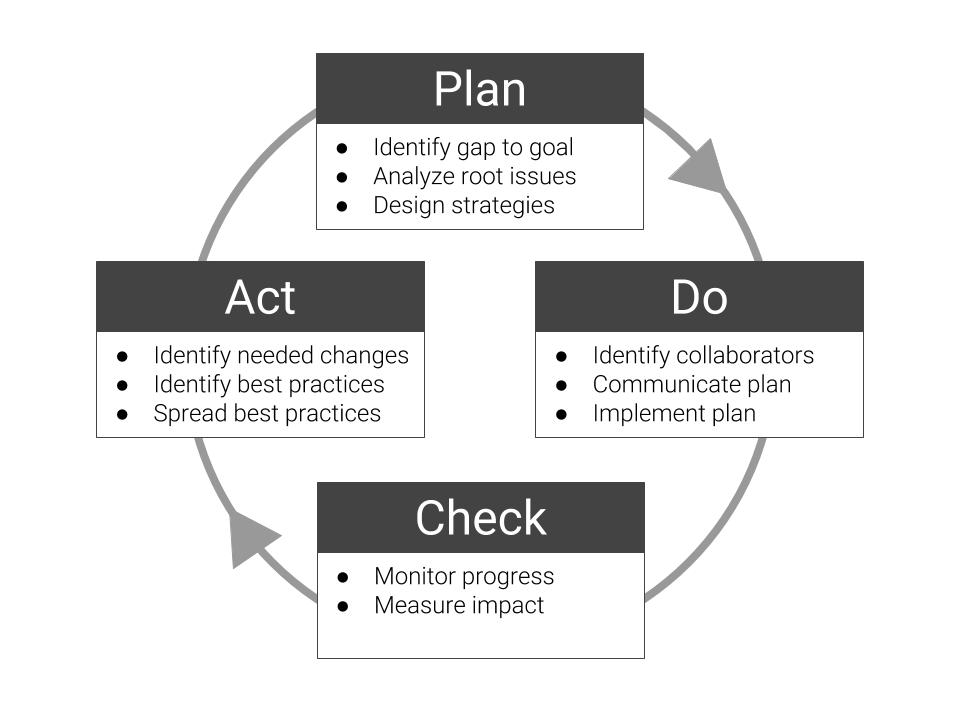
\includegraphics[width=24in]{_bookdown_files/img/pdca} \end{figure}

The table below illustrates the relationship between the PDCA process and a fuller definition of the PCP process:

\begin{table}

\caption{\label{tab:unnamed-chunk-3}Alignment of PDCA and PCP}
\centering
\begin{tabular}[t]{l|l|l|l|l}
\hline
Factor & Plan & Do & Check & Act\\
\hline
*Questions* & What is your life like? & What are you working on? & Is life better? & What next?\\
\hline
 & What do you want to pursue? & How are supports provided? &  & How to improve approach?\\
\hline
 & What supports do you need? & Where do you live/work? &  & \\
\hline
*Activities* & Identify QoL & Work on plan & Check QoL & Revise plan\\
\hline
 & Assess needs & Coordinate services & Reassess needs & (Repeat cycle)\\
\hline
 & Develop plan &  &  & \\
\hline
*Quality area* & Structure & Process & Outcome & (Re)structure\\
\hline
\end{tabular}
\end{table}

While there are various other rubrics related to learning and improvement, PDCA has been selected here because of its use of `planning' language, its simplicity, and its familiarity among behavioral healthcare providers and funders. Note that, while the questions above can be tied to various data-points, it is more important that they should be conversational: founded upon an ongoing process of personal striving for improvement.

\hypertarget{bok}{%
\chapter{A Common Body of Knowledge}\label{bok}}

A foundational effort has been working to develop a shared repository of key terms and concepts, their definitions, and how they are related to one another. This common language has the following key features:

\begin{itemize}
\tightlist
\item
  Relates all terminology back to the person, who is at the center
\item
  Includes concepts related to the PCP process, as broadly defined above, as well as common attributes for understanding the person\footnote{Note that the body of knowledge is not intended to classify services and supports.}
\item
  Promotes consistency in implementation and training, and the scalability of future development
\item
  Allows for change; the language can be extended as new concepts are identified.\footnote{This approach also requires that ideas claiming to be new must differentiate themselves from existing terms and concepts.}
\item
  Reduces confusion across various policies with inconsistent terminology and scope
\end{itemize}

\hypertarget{policy}{%
\chapter{Comprehensive Mapping to Policy}\label{policy}}

As with any important idea, person-centered planning has been discussed and debated for decades, leaving a vast body of policy, regulations, guidance, and explanations to sift through. While many of the basic ideas of person-centered planning are simple and commonsense, practitioners are also required to adhere to existing policies. With this in mind, the body of knowledge is being developed:

\begin{itemize}
\tightlist
\item
  Based on a broad scope of relevant state and federal policies identified by MDHHS-BHDDA.
\item
  Using natural-language processing techniques to identify and refine core terminology from the text of the identified policies
\item
  In a manner that allows MDHHS-BHDDA to identify whether new federal policies would align with the current implementation of PCP
\end{itemize}

\hypertarget{research}{%
\chapter{Informed by (and Informing) Research}\label{research}}

Some activities related to person-centered planning are addressed in existing research.\footnote{For instance, \emph{goals and planning}, \emph{feedback and monitoring}, and similar activities defined by the \href{https://www.humanbehaviourchange.org/resources/behavioural-science/25/description}{Behaviour Change Intervention Ontology (BCIO)} have related research available.} In these instances, our goal would be to connect-the-dots between research and practice by making this knowledge available. In order to remain aligned with national efforts\footnote{NQF's \href{http://www.qualityforum.org/WorkArea/linkit.aspx?LinkIdentifier=id\&ItemID=91382}{Person-Centered Planning and Practice Project}, references `\emph{a research agenda to advance and promote person-centered planning in LTSS}'} in this area, initial steps would include:

\begin{itemize}
\tightlist
\item
  mapping of person-centered planning concepts to researched interventions, where these exist
\item
  use of key concepts from the body of knowledge for literature review and meta-analyses of PCP-related practices, to build a base of best practices and evidence for effectiveness
\item
  identification of gaps in existing research knowledge related to PCP
\end{itemize}

\hypertarget{curriculum}{%
\chapter{Shared Training Curriculum}\label{curriculum}}

To translate this common body of knowledge into action, various audiences need to be trained in the core elements of person-centered practice, using the foundational concepts identified and defined above. Work in developing these trainings includes:

\begin{itemize}
\tightlist
\item
  Identification of key audiences
\item
  Evaluation of potential training modalities based on key features
\item
  Developing a standard base curriculum as well as specialty topics for specific audiences
\end{itemize}

\hypertarget{measure}{%
\chapter{Person-Centered Measurement Framework}\label{measure}}

If the entire system of services and supports is intended to be person-centered, its performance should be measured within a framework that is centered on the person. Since many existing quality measures and data collection systems were not developed with this in mind, it will be important to develop a larger framework within which existing measures can be situated. This allows the system to retain the quality measurement work that has been completed, while acknowledging gaps within that framework which need to be filled.

Ongoing work in this area would include:

\begin{itemize}
\tightlist
\item
  Developing a person-centered measurement framework
\item
  Conducting an inventory of available data assets at a state wide level
\item
  Classifying existing measurement and data collection efforts (e.g.~HEDIS, BH-TEDS, etc.) within the context of this framework
\end{itemize}

\hypertarget{what-do-we-mean-by-a-better-life}{%
\section{What do we mean by `a better life'?}\label{what-do-we-mean-by-a-better-life}}

People have been asking themselves what it means to live a good life for thousands of years,\footnote{The philosopher Aristotle defined the highest good of human life as happiness, or flourishing (\emph{eudaimonia}). cf.~\emph{Nicomachean Ethics}} and it is among the most crucial questions for each of us to answer. Here, we will refer to the characteristics that make up a good life as \emph{quality of life}, or QOL for short, relying primarily on contemporary research to arrive at a common and usable definition.

\hypertarget{what-makes-a-good-definition}{%
\subsection{What makes a good definition?}\label{what-makes-a-good-definition}}

If we are going to try to define quality of life, it is important that our definition gets a few things right:\footnote{These considerations are drawn from \href{https://www.ncbi.nlm.nih.gov/pubmed/16162114}{Cummins, R. (2005). Moving from the quality of life concept to a theory. JIDR, 49(10), 699-706}.}

\begin{enumerate}
\def\labelenumi{\arabic{enumi}.}
\tightlist
\item
  \emph{Multiple dimensions}. A good life can only be described using multiple dimensions. These are influenced by personal factors, environmental factors, and the interaction between those factors.
\item
  \emph{Broad enough for everyone}. We should each want to apply the definition to our own lives. The basic characteristics of a good life are the same for all people, regardless of culture, gender, disability, etc.
\item
  \emph{Both subjective and objective}. People have different priorities. While a definition can point to objective facts related to QoL, it must include the point-of-view of the person who is living their life from day to day. Each dimension of a QoL model may have both objectively and subjectively defined indicators.
\end{enumerate}

Taken together, the criteria listed above seek to balance the abstract with the specific to arrive at a definition which is well-rounded and understandable.

\hypertarget{what-makes-a-better-life}{%
\subsection{What makes a better life?}\label{what-makes-a-better-life}}

Keeping our key requirements in mind, we can draw from the broad reservoir of studies on QoL to find frameworks which are multi-dimensional\footnote{See systematic review of HRQoL recommending addition of individual and environmental characteristics: \href{https://www.ncbi.nlm.nih.gov/pmc/articles/PMC3548743/}{Bakas, T., et al.~(2012)}.}, cross-culturally relevant,\footnote{See \href{https://www.researchgate.net/profile/Mian_Wang4/publication/7801771_Cross-Cultural_Study_of_Quality_of_Life_Indicators/links/0deec52df448eac34d000000/Cross-Cultural-Study-of-Quality-of-Life-Indicators.pdf}{Schalock, R., et al.~(2005).}.} and which provide both subjective and objective indicators.

Below is a potential model listing essential dimensions of QoL:

\begin{table}

\caption{\label{tab:unnamed-chunk-4}QoL Dimensions}
\centering
\begin{tabular}[t]{l|l|l}
\hline
Area & Dimension & Example Indicators\\
\hline
Independence & Personal development & Education status, personal skills, ADLs, IADLs\\
\hline
 & Self-determination & Choices, autonomy, personal control, goals\\
\hline
Social participation & Interpersonal relations & Social networks, activities, relationships\\
\hline
 & Social inclusion & Community integration, participation, roles\\
\hline
 & Rights & Human (respect/dignity, equality), Legal\\
\hline
Well-being & Emotional well-being & Safety, positive experiences, self-concept, stress\\
\hline
 & Physical well-being & Health, nutrition, recreation/physical exertion\\
\hline
 & Material well-being & Financial status, employment, housing, possessions\\
\hline
\end{tabular}
\end{table}

Please note that the framework listed above is one of many potential models, each of which contains many of the same basic dimensions, and many were developed with populations having specific conditions. Some other broad-based models for review include:

\begin{itemize}
\tightlist
\item
  The \href{https://apps.who.int/iris/bitstream/handle/10665/77932/WHO_HIS_HSI_Rev.2012.03_eng.pdf?sequence=1\&isAllowed=y}{World Health Organization Quality of Life (WHOQOL)} domains.
\item
  The \href{https://ec.europa.eu/eurostat/statistics-explained/index.php?title=Quality_of_life_indicators}{Eurostat QoL indicators} show an example of QoL domains applied for entire countries alongside financial indicators such as gross domestic product (GDP).
\item
  Healthy People 2020 has selected a subset of measures for monitoring health-related QoL and well-being in the United States. See their \href{https://www.healthypeople.gov/sites/default/files/HRQoLWBFullReport.pdf}{Foundation Health Measure Report: Health-Related QoL and Well-Being}.
\end{itemize}

\hypertarget{benefits-of-a-qol-perspective}{%
\section{Benefits of a QoL Perspective}\label{benefits-of-a-qol-perspective}}

\hypertarget{what-other-frameworks-exist}{%
\subsection{What other frameworks exist?}\label{what-other-frameworks-exist}}

One might well ask: \emph{Is quality of life the only potential framework that we could use to measure improvement?} The answer is \emph{No}, so it is worth discussing other options and briefly reviewing the attributes of each. Other options include:

\begin{itemize}
\tightlist
\item
  \emph{Symptom reduction}: Measurement of reduction in symptoms related to specific diagnosable conditions. Symptom scales such as the \href{https://www.phqscreeners.com/sites/g/files/g10049256/f/201412/PHQ-9_English.pdf}{PHQ-9}, \href{}{GAD-7} and other tools have commonly been used to measure the impact of treatments on specific conditions, but they are more challenging to use for people with multiple co-occuring conditions (MCC).
\item
  \emph{Improving functional status}: Most currently used assessment tools address functional status, measuring the impact of various conditions on broader life areas in terms of their impact on functional ability. These are broader than symptom scales, and can detect the impact of various symptoms on a particular functional domain.
\item
  \emph{Health-related quality of life (HRQoL)}: HRQoL addresses a subset of QoL domains which are related to perceived physical and mental health. These models typically exclude non-medical areas such as education or rights, focusing on physical domains like `mobility'.
\end{itemize}

\hypertarget{why-is-a-quality-of-life-framework-better-than-others}{%
\subsection{Why is a quality of life framework better than others?}\label{why-is-a-quality-of-life-framework-better-than-others}}

A QoL approach has the following benefits over the approaches mentioned above:

\textbf{Strengths-based}: A QoL approach asks people what they want their lives to be and encourages them to work toward that vision. Rather than focusing on needs or deficits, it aspires to use a person's strengths to improve his or her life.\footnote{See the MDHHS PCP Policy value that ``The PCP approach identifies the person's strengths, goals, choices\ldots{} and desired outcomes.'' (p.~4)}

\textbf{Inclusive}: Instruments and measures from each of the other areas can be used as a part of the QoL framework, since it is broad enough to include each of these areas, and they each contribute to it. A QoL approach does not neglect the value of functional gains or symptom reduction, but values these as contributors to overall quality of life. For instance, if a person experiences an alleviation of their depressive symptoms using the PHQ-9, this would be seen as contributing toward the individual's QoL in the area of `Emotional Well-being'.

\textbf{Contextual}: An approach which focuses on only a portion of an individual's life, such as mobility or anxiety symptoms, is likely to miss out on the bigger picture. It may also inadvertently create siloes among the individuals supporting the person. For instance, more recent evaluations have criticized the HRQoL approach as failing to ``sufficient emphasis on mental and social domains\ldots{}that are essential to people.''\footnote{Read \href{https://www.ncbi.nlm.nih.gov/pmc/articles/PMC4031380/}{Pietersma, S., et al.~(2013)} regarding domains of quality of life.} The broader focus on QoL which is proposed here is aligned with our evolving understanding of several areas, each of which stresses the critical relationship between each of us and our communities and surroundings:

\begin{itemize}
\tightlist
\item
  \emph{Social Determinants of Health} (SDoH): A vast and growing body of \href{https://www.cdc.gov/socialdeterminants/research/index.htm}{research} indicates that the places and conditions in which we live are intrinsically tied to the quality of our lives and the likelihood of achieving positive outcomes from the supports and services we receive.
\item
  \emph{Trauma-Informed Care}: More and more models for service provision, informed by research and by the lived experience of trauma survivors, are founded on the recognition that adverse events in our relationships and in our lived environment can have a profound and lifelong impact on our lives.\footnote{For a recent review of these models, see: \href{https://www.ncbi.nlm.nih.gov/pubmed/30079827}{Purtle, J. (2018). Trauma, Violence, \& Abuse}.}
\item
  \emph{Supports Paradigm}: A model, prevalent in the IDD supports system, that views a person's functioning as the match between their individual capacity and the environment in which they are expected to live and work.\footnote{See \href{https://www.ncbi.nlm.nih.gov/pubmed/19368481}{Thompson, et al.~(2009)} on conceptualizing support needs.} In this model, supports are viewed as a way to supplement the persons strengths and to help match those to the person's environment.
\end{itemize}

  \bibliography{book.bib,packages.bib}

\end{document}
